\documentclass{article}
\usepackage[T1]{fontenc}
\usepackage[polish]{babel}
\usepackage[utf8]{inputenc}
\usepackage{graphicx} % Required for inserting images
\usepackage{amsmath}
\usepackage{nccmath}
\usepackage{float}
\usepackage{listings} % code highlighting
\usepackage{xcolor}
\usepackage{hyperref}
\usepackage{setspace}

\definecolor{codegreen}{rgb}{0,0.6,0}
\definecolor{codegray}{rgb}{0.5,0.5,0.5}
\definecolor{codepurple}{rgb}{0.58,0,0.82}
\definecolor{backcolour}{rgb}{0.95,0.95,0.92}

\lstdefinestyle{mystyle}{
    backgroundcolor=\color{backcolour},
    commentstyle=\color{codegreen},
    keywordstyle=\color{magenta},
    numberstyle=\tiny\color{codegray},
    stringstyle=\color{codepurple},
    basicstyle=\ttfamily\footnotesize,
    breakatwhitespace=false,
    breaklines=true,
    captionpos=b,
    keepspaces=true,
    numbers=left,
    numbersep=5pt,
    showspaces=false,
    showstringspaces=false,
    showtabs=false, 
    tabsize=2
}

\lstset{style=mystyle}
\lstset{ % polish letters in code blocks
  literate={ą}{{\k a}}1
  		     {Ą}{{\k A}}1
           {ż}{{\. z}}1
           {Ż}{{\. Z}}1
           {ź}{{\' z}}1
           {Ź}{{\' Z}}1
           {ć}{{\' c}}1
           {Ć}{{\' C}}1
           {ę}{{\k e}}1
           {Ę}{{\k E}}1
           {ó}{{\' o}}1
           {Ó}{{\' O}}1
           {ń}{{\' n}}1
           {Ń}{{\' N}}1
           {ś}{{\' s}}1
           {Ś}{{\' S}}1
           {ł}{{\l}}1
           {Ł}{{\L}}1
}

\title{MOwNiT - Laboratorium 3: \\
Interpolacja}
\author{Wojciech Dąbek}
\date{19 marca 2024}

\begin{document}

\maketitle

\section{Treści zadań laboratoryjnych}

\begin{enumerate}
    \item Dane są trzy węzły interpolacji: \((-1,2.4),\ (1,1.8),\ (2,4.5)\). Proszę obliczyć wielomian interpolacyjny 2-go stopnia, wykorzystując:
    \begin{itemize}
        \item jednomiany
        \item wielomiany Lagrange’a
        \item wielomiany wg wzoru Newtona
    \end{itemize}
    Proszę pokazać, że trzy reprezentacje dają ten sam wielomian.
    \item Wyrazić następujący wielomian metodą Hornera: \(p(t) = 3t^3 - 7t^2 + 5t - 4\)
    \item Ile mnożeń trzeba wykonać do ewaluacji  wielomianu \(p(t)\) stopnia \(n-1\) w danym punkcie \textit{t} jeżeli wybieramy jako reprezentacje:
    \begin{itemize}
        \item jednomiany
        \item wielomiany Lagrange’a
        \item wielomiany Newtona
    \end{itemize}
\end{enumerate}

\section{Treści zadań domowych}

\begin{enumerate}
    \item Znaleźć kompromis między granicą błędu a zachowaniem wielomianu interpolacyjnego dla funkcji Rungego \(f(t) = \frac{1}{1 + 25t^2}\), dla równoodległych węzłów na przedziale \([-1,1]\).
    \item Proszę:
    \begin{itemize}
        \item sprawdzić, czy pierwsze siedem wielomianów Legendre’a są wzajemnie ortogonalne
        \item sprawdzić, czy one spełniają wzór na rekurencję
        \item wyrazić każdy z sześciu pierwszych jednomianów \(1,\ t,\ \ldots,\ t^6\)\\
        jako liniową kombinację pierwszych siedmiu wielomianów Legendre’a \(p_0,\ \ldots,\ p_6\).
    \end{itemize}
    \item Dana jest funkcja określona w trzech punktach \(x_0,\ x_1,\ x_2\), rozmieszczonych w jednakowych odstępach \((x_1 = x_0 + h,\ x_2 = x_1 + h)\):
      \[f(x_0) = y_0,\ f(x_1) = y_1,\ f(x_2) = y_2\]
    Proszę wykonać interpolację danej funkcji sklejanymi funkcjami sześciennymi.
\end{enumerate}

\section{Rozwiązania zadań laboratoryjnych}

\subsection{}
\begin{itemize}
    \item Wykorzystując jednomiany:\\
    Współczynniki \(a_j\) postaci naturalnej szukanego wielomianu interpolacyjnego 2-go stopnia można wyznaczyć rozwiązując układ równań:
    \[f(x_i) = \sum_{j=0}^2 a_j x_i^j \text{ dla } i = 0, 1, 2\]
    Podstawiam zadane węzły interpolacji:
    \[\left\{
    \begin{array}{l}
         a_0 - a_1 + a_2 = 2.4\\
         a_0 + a_1 + a_2 = 1.8\\
         a_0 + 2a_1 + 4a_2 = 4.5
    \end{array}
    \right.
    \Rightarrow\ 
    \left\{
    \begin{array}{l}
         a_0 = 1.1\\
         a_1 = -0.3\\
         a_2 = 1
    \end{array}
    \right.\]
    Szukany wielomian ma zatem postać:
    \[\boldsymbol{x^2 - 0.3x + 1.1}\]
    \item Wykorzystując wielomiany Lagrange’a:
    \begin{gather*}
        P_2(x) = \sum_{k=0}^2 f(x_k) L_k(x) \quad \text{gdzie} \quad L_k(x) = \prod_{i = 0, i \neq k}^2 \frac{x - x_i}{x_k - x_i}\\
        P_2(x) = y_0 \frac{(x-x_1)(x-x_2)}{(x_0-x_1)(x_0-x_2)} + y_1 \frac{(x-x_0)(x-x_2)}{(x_1-x_0)(x_1-x_2)} + y_2 \frac{(x-x_0)(x-x_1)}{(x_2-x_0)(x_2-x_1)}
    \end{gather*}
    Podstawiam zadane węzły interpolacji:
    \begin{align*}
        P_2(x) &= 2.4 \frac{(x-1)(x-2)}{(-1-1)(-1-2)} + 1.8 \frac{(x-(-1))(x-2)}{(1-(-1))(1-2)} + 4.5 \frac{(x-(-1))(x-1)}{(2-(-1))(2-1)} =\\
        &= 0.4(x-1)(x-2) -0.9(x+1)(x-2) + 1.5(x+1)(x-1) =\\
        &= \boldsymbol{x^2 - 0.3x + 1.1}
    \end{align*}
    \item Wykorzystując wielomiany Newtona:
    \[P_2(x) = f[x_0] + f[x_0, x_1](x-x_0) + f[x_0,x_1,x_2](x-x_0)(x-x_1)\]
    Podstawiam do obliczeń zadane węzły interpolacji:
    \begin{gather*}
        f[x_0] = f(x_0) = 2.4\\
        f[x_0, x_1] = \frac{f[x_1] - f[x_0]}{x_1 - x_0} = \frac{1.8 - 2.4}{1 + 1} = -0.3\\
        f[x_1, x_2] = \frac{f[x_2] - f[x_1]}{x_2 - x_1} = \frac{4.5 - 1.8}{2 - 1} = 2.7\\
        f[x_0, x_1, x_2] = \frac{f[x_1, x_2] - f[x_0, x_1]}{x_2 - x_0} = \frac{2.7 + 0.3}{2 + 1} = 1
    \end{gather*}
    Stąd mamy:
    \begin{align*}
        P_2(x) &= 2.4 - 0.3(x+1) + (x+1)(x-1) =\\
        &= \boldsymbol{x^2 - 0.3x + 1.1}
    \end{align*}
\end{itemize}
\textbf{Wniosek:} Wszystkie trzy metody dają ostatecznie ten sam wielomian interpolacyjny.

\subsection{}
Dokonując odpowiednich przekształceń otrzymujemy:
\[p(t) = 3t^3 - 7t^2 + 5t - 4 = t(3t^2 - 7t + 5) - 4 = t(t(3t - 7) + 5) - 4 = t(t(t\ \cdot\ 3 - 7) + 5) - 4\]

\subsection{}
\begin{itemize}
    \item Wybierając jednomiany, możemy zastosować algorytm Hornera dla postaci naturalnej. Przy jego użyciu do ewaluacji wielomianu stopnia \(n-1\) wykonywanych jest \(n-1\) mnożeń.
    \item Wybierając wielomiany Lagrange’a, przy każdej ewaluacji wartości w konkretnym punkcie musimy powtórzyć obliczanie licznika dla każego \(L_k(x)\), co daje \(n-1\) mnożeń do wykonania \textit{n} razy. Oprócz tego, każdą obliczoną bazę Lagrange’a mnożymy jeszcze przez odpowiedni współczynnik (rzędną węzła), co daje kolejne \textit{n} mnożeń. Stąd przy takiej ewaluacji wykonywanych jest ich \(n(n-1) + n = n^2\).
    \item Wybierając wielomiany Newtona, obliczamy \(n-1\) kolejnych wartości \(p_k(x),\)
    \(k \in [1, n-1]\), które wymagają wykonania \(k-1\) mnożeń. Każdy z nich mnożymy jeszcze przez odpowiedni współczynnik \(b_k\). Stąd mamy w sumie \(\sum_{k=1}^{n-1} (k-1)+1 = \sum_{k=1}^{n-1} k = \frac{1}{2}(n-1)n\) mnożeń.
\end{itemize}

\section{Rozwiązania zadań domowych}

\subsection{}
Poniższy program napisany w języku Python generuje wykresy funkcji Rungego i jej wielomianu interpolacyjnego dla \(n = 4,\ 5,\ \ldots,\ 12\) równoodległych węzłów na przedziale \([-1, 1]\).
\begin{lstlisting}[language=Python]
import numpy as np
from matplotlib import pyplot
from scipy import interpolate


def runge(t) -> float:
    return 1 / (1 + 25 * t * t)


x = np.linspace(-1, 1, 1000)


def plot_for_n_knots(n: int):
    x_knots = np.linspace(-1, 1, n)
    y_knots = runge(x_knots)
    y = interpolate.krogh_interpolate(x_knots, y_knots, x)

    pyplot.title(f'Wykres dla {n} węzłów')
    pyplot.plot(x_knots, y_knots, 'o', label='węzły')
    pyplot.plot(x, y, label='interpolująca')
    pyplot.plot(x, runge(x), label='interpolowana')
    pyplot.legend()
    pyplot.show()


if __name__ == '__main__':
    for n in range(4, 13):
        plot_for_n_knots(n)
\end{lstlisting}

\begin{figure}[H]
    \centering
    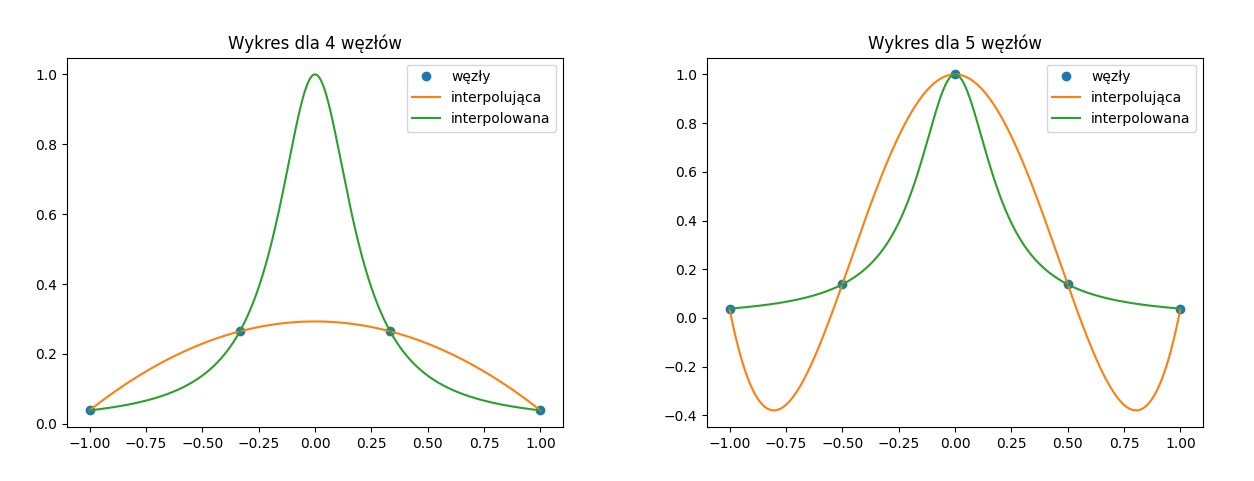
\includegraphics[width=\linewidth]{wykresy1.png}
\end{figure}
\begin{figure}[H]
    \centering
    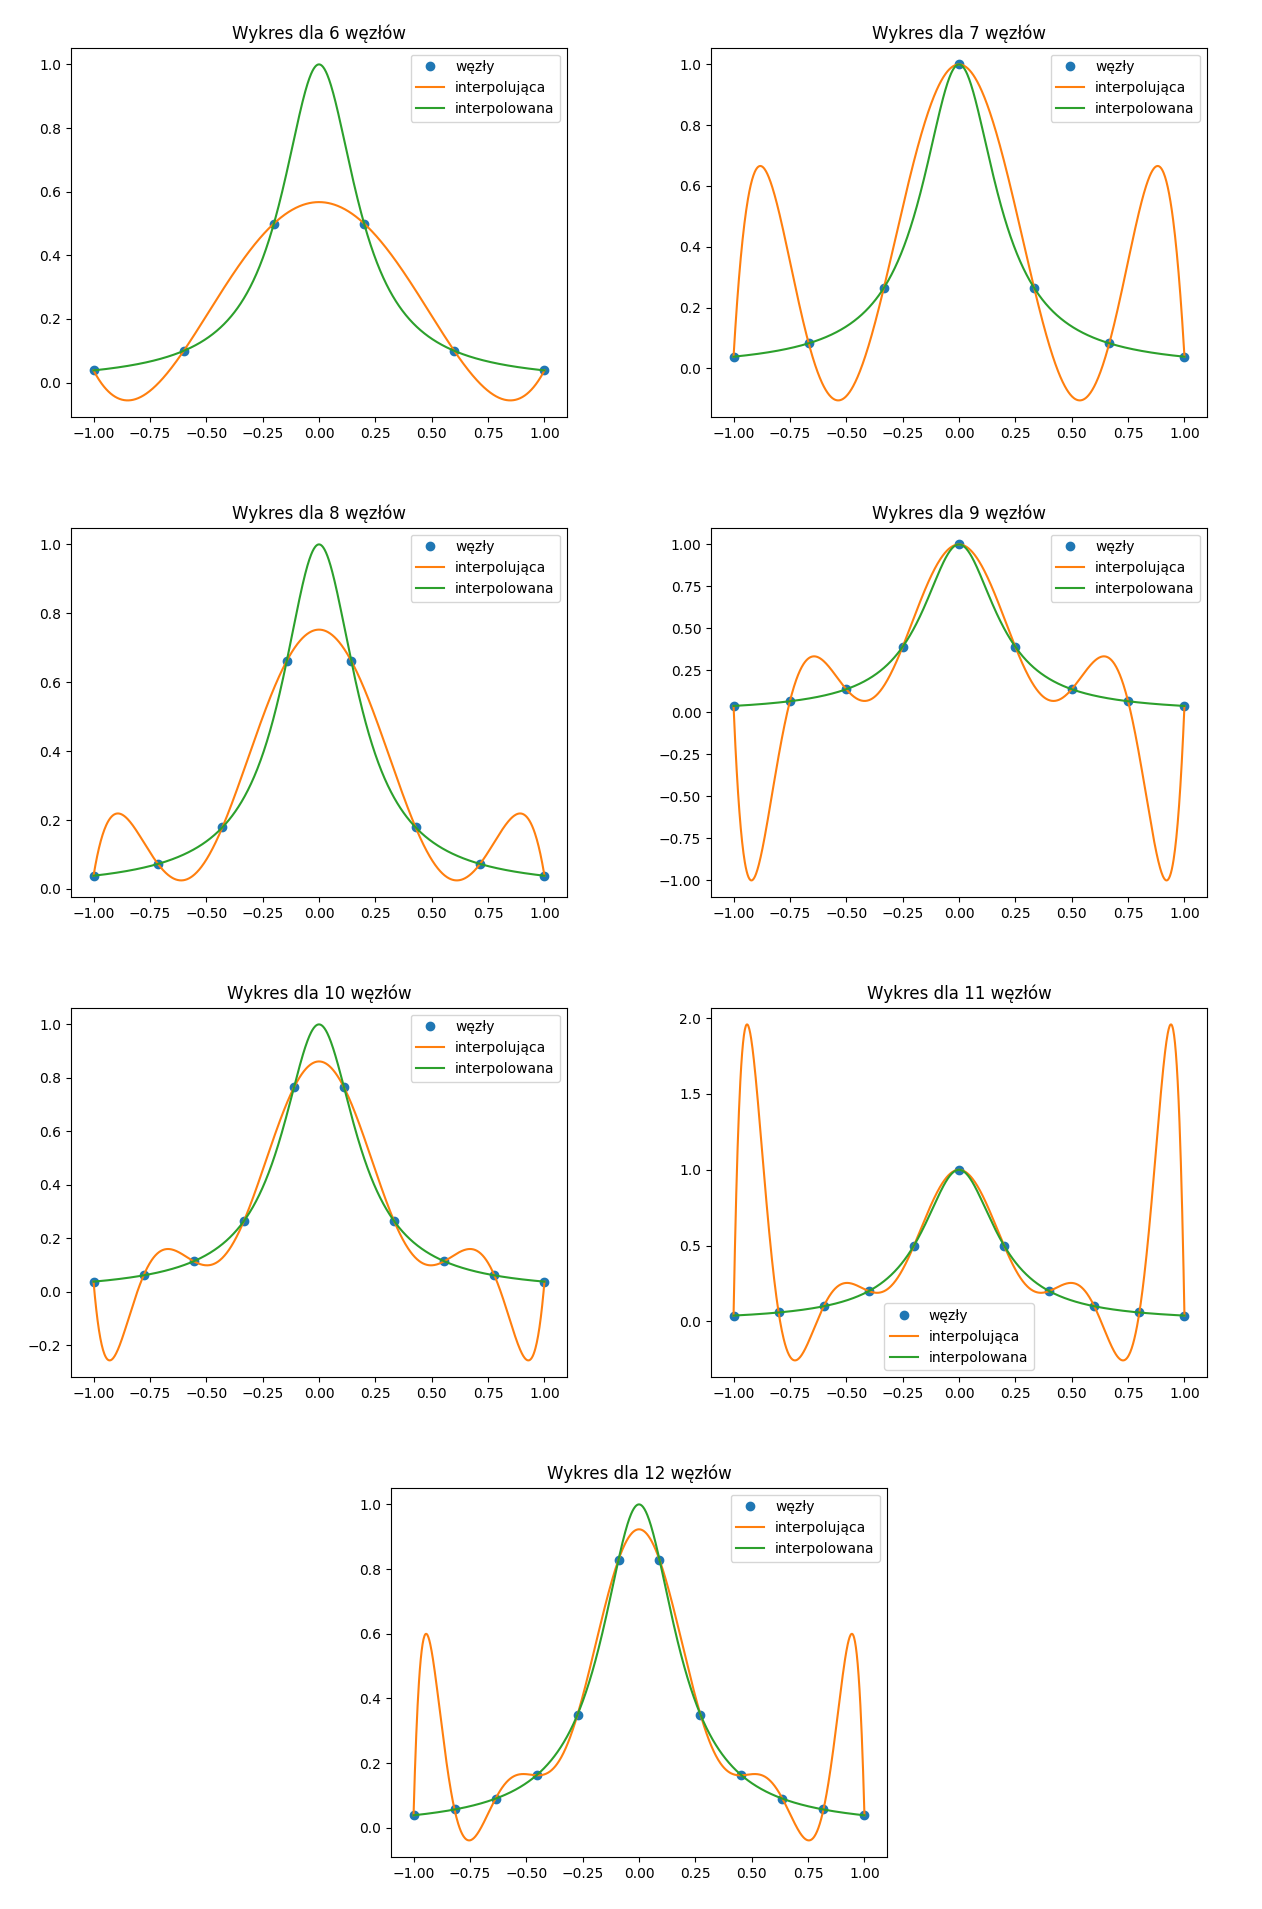
\includegraphics[width=\linewidth]{wykresy2.png}
\end{figure}

\newpage
\noindent
Początkowo można zauważyć wyraźnie mniejsze rozbieżności wykresów funkcji interpolującej od interpolowanej dla parzystej liczby węzłów, ale dla \(n \geq 12\) są one i tak bardzo duże.

\vspace{3mm}
\noindent
\textbf{Wniosek:} Jako rozsądny kompromis przyjmuję \(n = 10\) węzłów.

\subsection{}
\begin{itemize}
    \item Pierwsze 7 wielomianów Legendre'a:
    
    \setstretch{1.25}
    \(P_0(x) = 1\)\\
    \(P_1(x) = x\)\\
    \(P_2(x) = \frac{1}{2}(3x^2 - 1)\)\\
    \(P_3(x) = \frac{1}{2}(5x^3 - 3x)\)\\
    \(P_4(x) = \frac{1}{8}(35x^4 - 30x^2 + 3)\)\\
    \(P_5(x) = \frac{1}{8}(63x^5 - 70x^3 + 15x)\)\\
    \(P_6(x) = \frac{1}{16}(231x^6 - 315x^4 + 105x^2 - 5)\)
    
    \setstretch{1}
    Licząc dla każdej kombinacji różnych od siebie powyższych wielomianów całkę
    \[\int_{-1}^1 P_i(x)P_j(x)\ dx\]
    zawsze otrzymamy zero, co z definicji oznacza ich wzajemną ortogonalność.

    Dla potwierdzenia obliczeń dokonywanych najpierw w silniku obliczeniowym \textit{Wolfram|Alpha}, posłużyłem się następującym programem w języku R:
\begin{lstlisting}[language=R]
p <- function(i, x) {
  if (i == 0) return(1)
  if (i == 1) return(x)
  return(((2*i+1)/(i+1))*x*p(i-1,x) - (i/(i+1))*p(i-2, x))
}

pp <- function(i, j, x) {
  return(p(i, x) * p(j, x))
}

for (i in 0:6) {
  for (j in 0:6) {
    if (i == j) next
    ppv <- Vectorize(function(x) pp(i, j, x))
    print(integrate(ppv, -1, 1))
  }
}
\end{lstlisting}
    Program ten wypisał dla wszystkich rozważanych kombinacji wynik kwadratur jako dokładnie 0 lub niemalże 0 (z uwagi na niedokładność obliczeń na liczbach zmiennoprzecinkowych i aproksymacyjną naturę kwadratur).

    \newpage
    \noindent
    Obliczeń tych może być wyraźnie mniej przy zauważeniu, że każdy wielomian o nieparzystym numerze \((P_1, P_3, \ldots)\) jest nieparzysty, a każdy o parzystym - parzysty. Iloczyn funkcji nieparzystej z parzystą jest zawsze nieparzysty, a więc całkuje się do 0 na symetrycznym przedziale względem 0, tak jak w tym przypadku.

    \item Wzór rekurencyjny wygląda następująco:
    \[\left\{
    \begin{array}{l}
         P_{n+1}(x) = \frac{2n+1}{n+1}xP_n(x) - \frac{n}{n+1}P_{n-1}(x)\\
         P_0(x) = 1\\
         P_1(x) = x
    \end{array}
    \right.\]
    Następujący program w języku Python oblicza kolejne wyrazy ciągu rekurencyjnego.
\begin{lstlisting}[language=Python]
from numpy.polynomial.polynomial import Polynomial


p = [Polynomial([1]), Polynomial([0, 1])]
x = Polynomial([0, 1])  # x jako wielomian 0 + 1*x

for n in range(1, 6):
    p.append((2*n + 1)/(n+1) * x * p[n] - n/(n+1) * p[n-1])
    print(p[n+1])
\end{lstlisting}
    Program wypisał takie reprezentacje obliczonych wielomianów:
\begin{verbatim}
-0.5 + 0.0 x + 1.5 x**2
0.0 - 1.5 x + 0.0 x**2 + 2.5 x**3
0.375 + 0.0 x - 3.75 x**2 + 0.0 x**3 + 4.375 x**4
0.0 + 1.875 x + 0.0 x**2 - 8.75 x**3 + 0.0 x**4 + 7.875 x**5
-0.3125 + 0.0 x + 6.5625 x**2 + 0.0 x**3 - 19.6875 x**4
                              + 0.0 x**5 + 14.4375 x**6
\end{verbatim}
    Odpowiadają one wielomianom podawanym w tablicach, więc zależność rekurencyjna jest spełniona.

    \item Kombinacji liniowych wielomianów Legendre'a odpowiadających pierwszym jednomianom można łatwo szukać znając już rozwiązania dla niższych numerów wielomianów. Zaczynam więc od zanotowania \(1 = P_0\).\\
    Idąc dalej:
    \begin{align*}
        &t = P_1\\
        2P_2 = 3t^2 - 1 \Rightarrow\ &t^2 = \frac{1}{3}(2P_2 + P_0)\\
        2P_3 = 5t^3 - 3t \Rightarrow\ &t^3 = \frac{1}{5}(2P_3 + 3P_1)\\
        8P_4 = 35t^4 - 30t^2 + 3 \Rightarrow\ &t^4 = \frac{1}{35}(8P_4 + 20P_2 + 7P_0)\\
        8P_5 = 63t^5 - 70t^3 + 15t \Rightarrow\ &t^5 = \frac{1}{63}(8P_5 + 28P_3 + 27P_1)\\
        16P_6 = 231t^6 - 315t^4 + 105t^2 - 5 \Rightarrow\ &t^6 = \frac{1}{231}(16P_6 + 72P_4 + 110P_2 + 103P_0)
    \end{align*}
\end{itemize}

\subsection{}
Konstruuję funkcję
\[s(x) =
\begin{cases}
    s_0(x) & x \in [x_0,\ x_1]\\
    s_1(x) & x \in [x_1,\ x_2]
\end{cases}
\]
spełniającą warunki interpolacji funkcji \textit{f} dla zadanych węzłów, w której funkcje \(s_0\) i \(s_1\) są sześcienne. Wiadomo stąd, że ich drugie pochodne \(s_i''\) są liniowe na swoich przedziałach. Łącząc to z warunkiem interpolacji sześciennej\\
\(s_i''(x_{i+1}) = s_{i+1}''(x_{i+1})\), dla \(i \in \{0, 1\}\) otrzymuję wzór:
\[s_i''(x) = s_i''(x_i) \frac{x_{i+1} - x}{h} + s_i''(x_{i+1}) \frac{x - x_i}{h}\]
Całkując dwukrotnie otrzymuję:
\[s_i(x) = \frac{s_i''(x_i)}{6h}(x_{i+1} - x)^3 + \frac{s_i''(x_{i+1})}{6h}(x - x_i)^3 + C(x - x_i) + D(x_{i+1} - x)\]
gdzie \(C \text{ i } D\) to stałe całkowania, które mogę wyliczyć korzystając z warunków interpolacji \(s_i(x_i) = y_i\) oraz \(s_i(x_{i+1}) = y_{i+1}\). Dzięki temu mamy:
\begin{align*}
    s_i(x) &= \frac{s_i''(x_i)}{6h}(x_{i+1} - x)^3 + \frac{s_i''(x_{i+1})}{6h}(x - x_i)^3 +\\
    &+ \left(\frac{y_{i+1}}{h} - \frac{s_i''(x_{i+1})h}{6}\right)(x - x_i) + \left(\frac{y_i}{h} - \frac{s_i''(x_i)h}{6}\right)(x_{i+1} - x)
\end{align*}
Do wyliczenia \(s_i''(x)\) skorzystam z warunku ciągłości pierwszej pochodnej.\\
Różniczkując powyższą funkcję na przedziale otrzymuję:
\[s_i'(x_i) = -\frac{h}{3}s_i''(x_i) - \frac{h}{6}s_i''(x_{i+1}) + \frac{y_{i+1} - y_i}{h}\]
Dla przejrzystości wprowadzam symbole:
\begin{align*}
    \sigma_i &= \frac{1}{6}s''(x_i) \left(= \frac{1}{6}s_0''(x_i) = \frac{1}{6}s_1''(x_i)\right)\\
    \Delta_i &= \frac{y_{i+1} - y_i}{h}
\end{align*}
Wtedy:
\begin{align*}
    s_1'(x_1) &= \Delta_1 - h(\sigma_2 + 2\sigma_1)\\
    s_0'(x_1) &= \Delta_0 + h(2\sigma_1 + \sigma_0) \text{ (wyznaczane analogicznie dla } s_{i-1})
\end{align*}
muszą być sobie równe:
\begin{gather*}
    \Delta_1 - h(\sigma_2 + 2\sigma_1) = \Delta_0 + h(2\sigma_1 + \sigma_0)\\
    h(\sigma_0 + 4\sigma_1 + \sigma_2) = \Delta_1 - \Delta_0
\end{gather*}
Mamy w jednym równaniu trzy niewiadome, więc koniecznie jest określenie warunków brzegowych, dlatego przyjmuję \(s''(x_0) = s''(x_2) = 0\ (= \sigma_0 = \sigma_2)\) (\textit{natural cubic spline}). Pozostaje wtedy:
\begin{gather*}
    4h\sigma_1 = \Delta_1 - \Delta_0\\
    4h\sigma_1 = \frac{y_0 - 2y_1 + y_2}{h}\\
    \sigma_1 = \frac{y_0 - 2y_1 + y_2}{4h^2}
\end{gather*}
Ostateczną postać funkcji interpolującej \textit{s} otrzymamy podstawiając współrzędne węzłów interpolacji oraz wartości \(\sigma_i\) do wzoru:
\[s(x) = 
\begin{cases}
    y_0 + b_0(x - x_0) + c_0(x - x_0)^2 + d_0(x - x_0)^3, & x \in [x_0,\ x_1]\\
    y_1 + b_1(x - x_1) + c_1(x - x_1)^2 + d_1(x - x_1)^3, & x \in [x_1,\ x_2]
\end{cases}
\]
gdzie
\begin{align*}
    b_i &= \frac{y_{i+1} - y_i}{h} - h(\sigma_{i+1} + 2\sigma_i)\\
    c_i &= 3\sigma_i\\
    d_i &= \frac{\sigma_{i+1} - \sigma_i}{h}
\end{align*}

\section{Bibliografia}
Wykład \textit{MOwNiT - Interpolacja} - Marian Bubak, Katarzyna Rycerz\\
Wykład \textit{MOwNiT - Funkcje sklejane - spline functions} - Marian Bubak, Katarzyna Rycerz\\
Dokumentacja \href{https://docs.scipy.org/doc/scipy/reference/generated/scipy.interpolate.krogh_interpolate.html#scipy.interpolate.krogh_interpolate}{\textit{SciPy Manual}}\\
Dokumentacja \href{https://numpy.org/doc/stable/reference/generated/numpy.polynomial.polynomial.Polynomial.html#numpy.polynomial.polynomial.Polynomial}{\textit{NumPy}}

\end{document}
